\section{Estado del arte}
\label{ch:2:section:state-of-the-art}

\subsection{La ciencia de datos}
% region subsection La ciencia de datos

La ciencia de datos (\textit{Data Science}) es el estudio de los datos con el objetivo de extraer información útil, se usa principalmente para dar información útil a empresas. Es un campo multidisciplinar, ya que combina campos de las matemáticas, estadística e inteligencia artificial para analizar grandes cantidades de datos. Esto tiene como objetivo responder a las siguientes cuestiones: \textit{¿Qué paso?, ¿Por qué pasó?, ¿Qué pasará? O ¿Qué se puede hacer con los resultados?} \cite{aws-data-science}

La ciencia de datos analiza los datos de distintas formas.

\begin{enumerate}
    \item \textbf{Análisis descriptivo}: examina datos con visualizaciones (gráficos, tablas) para entender eventos pasados o actuales.
    \item \textbf{Análisis de diagnóstico}: profundiza en los datos para entender las razones detrás del evento. Emplea técnicas como descubrimiento de datos o correlaciones.
    \item \textbf{Análisis predictivo}: utiliza datos históricos y técnicas como machine learning para hacer predicciones precisas sobre patrones futuros.
    \item \textbf{Análisis prescriptivo}: busca la mejor respuesta para un resultado esperado. Utiliza técnicas como simulación y redes neuronales para recomendar el mejor curso de acción entre varias alternativas.
\end{enumerate}

% endregion subsection La ciencia de datos

\subsection{La minería de datos}
% region subsection La minería de datos
% Fases de la extracción del conocimiento 
% Dentro del KDD está la {minería de datos}

La minería de datos, es una técnica asistida por computadora, procesa grandes conjuntos de datos para descubrir patrones y relaciones ocultas. Este conocimiento resultante se aplica en la resolución de problemas, análisis de decisiones empresariales, etc. Esta técnica tiene distintas fases para procesar y extraer información útil.

\begin{enumerate}
    \item Comprender, identificar y definir el alcance del proyecto.
    \item Comprender los datos.
    \item Depurar datos (limpiar, integrar y dar formato).
    \item Modelar datos.
    \item Evaluar los resultados.
    \item Implementar resultados.
\end{enumerate}

La minería de datos es distinta en función de los datos y el objetivo, la mayoría del estado del arte segmenta la minería en tres tipos, minería de procesos, minería de textos y minería predictiva.

El Descubrimiento de Conocimientos en Bases de Datos \gls{KDD} es un proceso que utiliza algoritmos de minería de datos para explorar y extraer conocimientos útiles de grandes bases de datos. Con el avance tecnológico, se emplean técnicas de inteligencia artificial para este propósito, con el objetivo final de obtener conocimiento de alto nivel a partir de datos de bajo nivel. La Figura \ref{fig:kdd} esquematiza el proceso general del \textit{KDD}.

\begin{figure}[H]
    \centering
    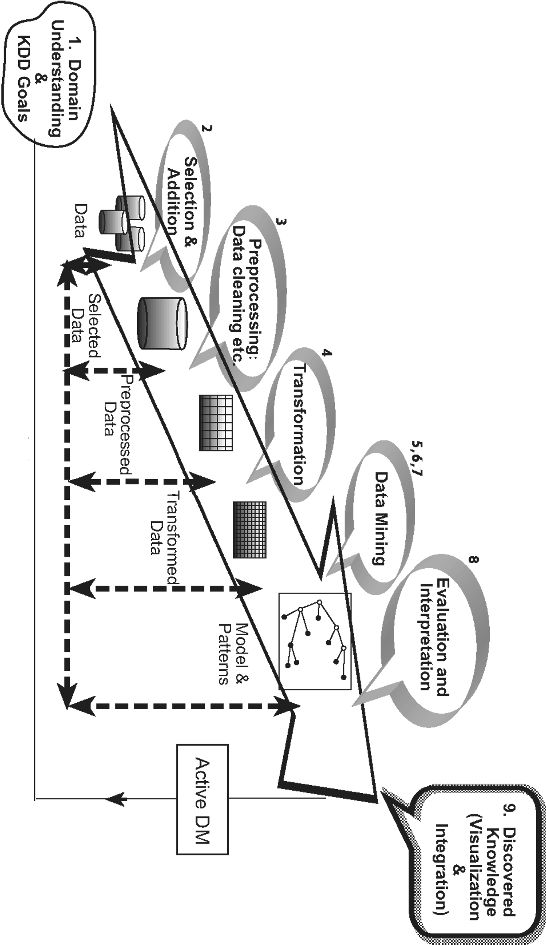
\includegraphics[angle=90,width=0.8\textwidth]{figures/chapter02/KDD.jpg}
    \caption{El proceso de descubrimiento de conocimiento en bases de datos.\newline{}Fuente: Sección \textit{Introduction to Knowledge Discovery and Data Mining} \cite{rokach2010data}}
    \label{fig:kdd}
\end{figure}

\begin{enumerate}
    \item \textbf{Comprensión del Dominio de Aplicación}: se debe comprender los datos que se tratan y el campo de obtención con el objetivo de preparar los datos.
    \item \textbf{Selección y Creación de Conjunto de Datos}: se han de seleccionar los datos relevantes (Selección de características).
    \item \textbf{Preprocesamiento y Limpieza de Datos}: se han de eliminar las características no relevantes, datos perturbados, entradas incoherentes o tratar datos faltantes, etc. con el objetivo de obtener datos más limpios.
    \item \textbf{Transformación de Datos}: se deben tratar los datos, reduciendo la dimensionalidad, filtración, descomponiendo, etc. para que sea más sencillo el consumo de estos datos por una aplicación.
    \item \textbf{Elección de Tarea de Minería de Datos}: en función de los datos y del objetivo deberemos realizar una tarea (clasificación, regresión o agrupación), ya que en la minería de datos hay dos objetivos principales, \textbf{predicción} y \textbf{descripción}.
    \item \textbf{Elección del Algoritmo de Minería de Datos}: deberemos elegir entre los distintos algoritmos que se usan en la minería de datos, si buscamos precisión podemos usar redes neuronales, si buscamos explicabilidad podemos usar árboles de decisión.
    \item \textbf{Implementación del Algoritmo de Minería de Datos}: emplearemos el algoritmo seleccionado ajustando los parámetros para que nos del mejor resultado.
    \item \textbf{Evaluación de Patrones Minados}: debemos interpretar los resultados (reglas, confiabilidad, etc.) si no cumplen los objetivos que se buscaban en el primer paso deberemos reajustar toda la metodología, desde ajustar la selección de características a la interpretación o compresibilidad del modelo.
    \item \textbf{Utilización del Conocimiento Descubierto}: por último, debemos incorporar el conocimiento a los sistemas de toma de decisiones, este es el paso más importante, ya que con él podemos medir los efectos del conocimiento obtenido. Puede suceder que una vez implementado el modelo en sistema de producción pierda eficiencia si las condiciones reales son distintas a las de la creación del modelo.
\end{enumerate}

\begin{figure}[H]
    \centering
    \centerline{\includesvg[width=1\linewidth]{figures/chapter02/data-mining-taxonomy.drawio.svg}}
    \caption{Taxonomía de minería de datos.\newline{}Fuente: Elaboración propia, inspirado en la sección \textit{Introduction to Knowledge Discovery and Data Mining} \cite{maimon2005data}}
    \label{fig:data-mining-taxonomy}
\end{figure}

La minería de datos puede estar orientada a la verificación o al descubrimiento de patrones, se debe automatizar su identificación, pudiendo usar un enfoque predictivo o descriptivo. Para el descubrimiento se usa el aprendizaje inductivo, mientras que en el paso de verificación se ha de evaluar las hipótesis externas usando métodos estadísticos clásicos. La terminología clásica del aprendizaje automático está clasificado en supervisado (clasificación y regresión) y no supervisado (agrupamiento), aunque existen muchos más términos en la terminología moderna esto podemos analizarlo más en profundidad en el libro \textit{Data Mining and Knowledge Discovery Handbook} \cite{maimon2005data}.

% endregion subsection La minería de datos

\subsection{Aprendizaje automático - \textit{Machine Learning}}
% region subsection Aprendizaje automático

El \textit{machine learning} es la ciencia o rama de la inteligencia artificial que desarrolla, modelos estadísticos, desarrolla algoritmos que generalizan comportamientos y reconocen patrones. Es decir, hace posible el aprendizaje autónomo de las máquinas para realizar tareas sin la necesidad programar las instrucciones explícitamente. El \textit{machine learning} busca procesar grandes cantidades de datos e identificar patrones de datos de forma automática.

\begin{figure}[H]
    \centering
    \centerline{\includesvg[width=0.75\linewidth]{figures/chapter02/machine-learning-rules.drawio.svg}}
    \caption{El \textit{Machine Learning} como paradigma de programación.\newline{}Fuente: Elaboración propia}
    \label{fig:machine-learning-rules}
\end{figure}

Como podemos ver en la Figura \ref{fig:machine-learning-rules} en el paradigma clásico se necesitaba conocer el dominio de los datos y las reglas en profundidad y programar los descriptores de forma manual para procesar los datos. En el paradigma del \textit{machine learning} permite extraer esas reglas y patrones para procesar nuevos datos a partir de respuestas que conocíamos previamente, estas respuestas previas deben ser extraídas o validadas por expertos.

Una clasificación de las tareas del \textit{machine learning} lo podemos ver en la Figura \ref{fig:machine-learning}, esta clasificación está dividida en función de cómo se realiza el aprendizaje del modelo.

\begin{figure}[H]
    \centering
    \centerline{\includesvg[width=1\linewidth]{figures/chapter02/machine-learning.drawio.svg}}
    \caption{Clasificación de los algoritmos de aprendizaje automático.\newline{}Fuente: Elaboración propia}
    \label{fig:machine-learning}
\end{figure}

El \textit{machine learning} puede trabajar con datos estructurados y no estructurados, aunque estos últimos requieren un procesamiento previo para adaptarlos en un formato estructurado.

% endregion subsection Aprendizaje automático

\subsection{Aprendizaje profundo - \textit{Deep Learning}}
% region subsection Aprendizaje profundo
% TODO: Explicar el Deep Learning 
% https://idus.us.es/bitstream/handle/11441/90004/Centeno%20Franco%20Alba%20TFG.pdf
% https://learning.oreilly.com/library/view/neural-networks-and/9781492037354/ch01.html#idm139624964652336

El \textit{deep learning} es una rama del \textit{machine learning} que usa redes neuronales artificiales para analizar datos no lineales, estas redes imitan el comportamiento del cerebro humano, para esto suelen contar con arquitecturas complejas.
Se distingue del \textit{machine learning} por los tipos de datos con los que puede trabajar y por los métodos con los que hace que los modelos aprendan.

Otra de las características que diferencia al \textit{deep learning} del \textit{machine learning} es que elimina parte del procesamiento previo de datos, ya que sus algoritmos pueden ingerir y procesar datos no estructurados.


% endregion subsection Aprendizaje profundo